\chapter{Liquid Neural Network Design and Implementation}

\section{Design Overview}
This chapter outlines the implementation of the Liquid Neural Network (LNN) developed in PyTorch for sequential 2D time-series prediction. The architecture is based on the Liquid Time-Constant (LTC) neuron model, which simulates continuous-time dynamics through ordinary differential equations (ODEs) and shows properties of neural adaptability and temporal memory.

The aim of the implementation was to create a biologically-inspired, interpretable recurrent model with competitive performance on trajectory prediction tasks. Unlike conventional RNNs or LSTMs, the LNN is governed by time-continuous equations rather than discrete updates, providing finer control over neuronal dynamics.

\vspace{1em}
\noindent The following principles guided the design:
\begin{itemize}
    \item \textbf{Framework:} PyTorch was selected due to its flexible dynamic graph construction and ease of integrating custom layers with automatic differentiation.
    \item \textbf{Neuron Dynamics:} The neuron model was designed to emulate leaky integrate-and-fire (LIF) behaviour with added plasticity through modulated reversal potentials and conductances.
    \item \textbf{Time Unfolding:} Each forward pass of the LNN integrates over multiple internal time steps (ODE unfolds) to approximate the continuous-time solution, reflecting membrane voltage evolution.
    \item \textbf{Baseline Comparison:} To benchmark performance, identical training and evaluation protocols were implemented for alternative architectures (LSTM, TCN) using the same data.
\end{itemize}

The following sections document the architecture, neuron formulation, wiring strategy, training setup, and performance characteristics of the LNN.

\section{Wiring and Connectivity}
LNNs have a sparse and biologically motivated connectivity structure. To simulate the non-uniform and random nature of synaptic wiring observed in biological networks, a custom class named \texttt{RandomWiring} was implemented.

This class generates two adjacency matrices:
\begin{itemize}
    \item A \textbf{recurrent adjacency matrix} of shape $(n \times n)$ defining internal connections between neurons within the hidden layer.
    \item A \textbf{sensory adjacency matrix} of shape $(d_{\text{in}} \times n)$ which defines the input-to-hidden connectivity.
\end{itemize}
Each matrix contains continuous values sampled from a uniform distribution on $[0, 1]$, which are later used to create binary masks or to modulate weight strengths.

The \texttt{RandomWiring} class also generates reversal potentials:
\begin{itemize}
    \item \texttt{erev} for neuron-neuron connections.
    \item \texttt{sensory\_erev} for input-synapse connections.
\end{itemize}
These potentials are initialised from a uniform range $[-0.2, 0.2]$ and are treated as fixed, non-learnable parameters in this implementation.

\vspace{1em}
\noindent \textbf{Key features of the \texttt{RandomWiring} class:}
\begin{itemize}
    \item \textbf{Biological plausibility:} Fixed sparse masks emulate the limited number of active connections in real cortical microcircuits.
    \item \textbf{Randomised initialisation:} Each instantiation of \texttt{RandomWiring} results in a different network topology, allowing stochastic variation in experiments.
    \item \textbf{Separation of sensory and recurrent dynamics:} By decoupling the sensory and recurrent wiring, the model can explicitly distinguish between input-driven and internal dynamic behaviour.
\end{itemize}

\noindent Below is a simplified example of the \texttt{RandomWiring} class:
\begin{lstlisting}[language=Python, caption={Simplified RandomWiring class}]
class RandomWiring:
    def __init__(self, input_dim, output_dim, neuron_count):
        self.adjacency_matrix = np.random.uniform(0, 1, (neuron_count, neuron_count))
        self.sensory_adjacency_matrix = np.random.uniform(0, 1, (input_dim, neuron_count))
        
    def erev_initializer(self):
        return np.random.uniform(-0.2, 0.2, (neuron_count, neuron_count))

    def sensory_erev_initializer(self):
        return np.random.uniform(-0.2, 0.2, (input_dim, neuron_count))
\end{lstlisting}

\section{LTC Neuron Dynamics}
The core unit of the LNN is the \texttt{LIFNeuronLayer}, a custom PyTorch module that simulates the behaviour of leaky integrate-and-fire neurons (also known as liquid time-constant neurons). These neurons operate using a continuous-time dynamical model controlled by a first-order differential equation, capturing the evolution of membrane potentials in response to internal and external stimuli.

The model integrates over time using a discretised ODE solver implemented within the forward pass. Specifically, it unfolds the membrane update equation over a fixed number of steps (\texttt{ode\_unfolds}) using an Euler-like method.

\noindent The update rule is determined by the equation:
\[
v_t = \frac{c_m \cdot v_{t-1} + g_{\text{leak}} \cdot V_{\text{leak}} + I_{\text{syn}}}{c_m + g_{\text{leak}} + G_{\text{syn}} + \varepsilon}
\]
where:
\begin{itemize}
    \item $c_m$: membrane capacitance (learnable)
    \item $g_{\text{leak}}$: leak conductance (learnable)
    \item $V_{\text{leak}}$: leak reversal potential
    \item $I_{\text{syn}}$: synaptic current from sensory and recurrent inputs
    \item $G_{\text{syn}}$: total synaptic conductance
    \item $\varepsilon$: small stabilisation constant
\end{itemize}

\noindent Both sensory and recurrent synaptic activations are modelled using a sigmoid function with learnable $\mu$ (mean) and $\sigma$ (scale), followed by a softplus-modulated weight:
\[
\text{activation} = \text{Softplus}(W) \cdot \sigma\left( \frac{v - \mu}{\sigma} \right)
\]

\vspace{1em}
\noindent \textbf{Implementation Details:}
\begin{itemize}
    \item \textbf{Learnable Parameters:} All biophysical constants—capacitance, leak conductance, reversal potentials, synaptic weights—are learnable, providing flexibility in dynamic behaviour.
    \item \textbf{Softplus Regularisation:} Weights and conductances are passed through \texttt{Softplus} to enforce positivity while allowing gradients to flow smoothly during training.
    \item \textbf{ODE Unfolding:} The number of internal solver steps is fixed (\texttt{ode\_unfolds} = 12) to balance numerical precision with computational cost.
    \item \textbf{Sparsity Masks:} Both recurrent and sensory activations are element-wise masked using the adjacency matrices from \texttt{RandomWiring}, enforcing fixed sparsity throughout training.
\end{itemize}

\noindent Below is the ODE solver implementation within the \texttt{LIFNeuronLayer} class:
\begin{lstlisting}[language=Python, caption={Simplified LTC neuron forward method}]
def ode_solver(self, inputs, state, elapsed_time):
    v_pre = state
    for _ in range(self.ode_unfolds):
        synaptic_input = compute_synaptic_activation(v_pre)
        numerator = self.cm * v_pre + self.gleak * self.vleak + synaptic_input
        denominator = self.cm + self.gleak + synaptic_conductance
        v_pre = numerator / (denominator + self.epsilon)
    return v_pre
\end{lstlisting}
This allows neurons to respond to both present input and also to their internal temporal dynamics, mimicking continuous-time memory traces observed in biological neurons.

\section{Network Architecture}
The full Liquid Neural Network is constructed by embedding the LTC neuron layer within a recurrent wrapper, implemented as a custom \texttt{LTCRNN} module. This wrapper sequentially passes each time step of the input through the same \texttt{LIFNeuronLayer}, maintaining a hidden state that evolves over time. The resulting structure can be viewed as a biologically grounded alternative to traditional RNN cells.

At a high level, the architecture accepts an input tensor of shape $(B, T, d_{\text{in}})$, where $B$ is the batch size, $T$ is the sequence length, and $d_{\text{in}}$ is the input dimension (two in this case, corresponding to 2D spatial coordinates). For each time step $t$, the neuron layer receives the $t$-th slice of the sequence and updates the hidden state, generating a predicted output of shape $(B, T, d_{\text{out}})$.

\vspace{1em}
\linebreakparagraph{Design Considerations and Tradeoffs:}
\begin{itemize}
    \item \textbf{Hidden state dimensionality:} The number of LTC neurons (set via \texttt{hidden\_dim}) defines the model capacity. A lower number limits expressiveness but reduces overfitting risk and improves computational efficiency.
    \item \textbf{Output mapping:} Rather than applying a separate output layer, the voltage traces themselves are treated as predictions. This design allows direct interpretation of the membrane state as a continuous output signal.
    \item \textbf{Batch-first structure:} Following PyTorch conventions, all sequences are processed in batch-major form, allowing efficient tensor operations and GPU parallelism.
\end{itemize}

\noindent The architecture can be summarised as follows:
\begin{lstlisting}[language=Python, caption={Structure of the LTCRNN module}]
class LTCRNN(nn.Module):
    def __init__(self, wiring, input_dim, hidden_dim, output_dim):
        self.cell = LIFNeuronLayer(wiring)
        ...
        
    def forward(self, inputs):
        batch_size, seq_len, _ = inputs.size()
        states = torch.zeros(batch_size, self.hidden_dim)
        outputs = []
        for t in range(seq_len):
            out, states = self.cell(inputs[:, t, :], states)
            outputs.append(out)
        return torch.stack(outputs, dim=1)
\end{lstlisting}

The design maintains a clear separation between the continuous-time neuronal dynamics and the sequence-level integration logic. As a result, the architecture remains both modular and biologically interpretable, while still being compatible with modern deep learning tools.

\begin{figure}[H]
    \centering
    \begin{tikzpicture}[node distance=1.4cm and 2.6cm, every node/.style={transform shape}]
        % Input
        \node[draw, fill=blue!10, rounded corners, minimum width=2.8cm, minimum height=1cm] (input) {Input Sequence};

        % RNN Loop
        \node[draw, fill=orange!25, rounded corners, minimum width=2.8cm, minimum height=1cm, below=of input] (ltccell) {LTC Cell};
        \draw[->, thick] (input) -- (ltccell);

        % Hidden State
        \node[draw, fill=gray!20, minimum width=1.5cm, minimum height=0.8cm, right=1.8cm of ltccell] (hidden) {State};
        \draw[->, thick] (ltccell.east) -- (hidden.west) node[midway, above, font=\footnotesize] {V(t)};
        \draw[->, thick] (hidden.north) to[out=135, in=45] (ltccell.north);

        % Output
        \node[draw, fill=cyan!10, rounded corners, minimum width=2.8cm, minimum height=1cm, below=of ltccell] (output) {Predicted Output};
        \draw[->, thick] (ltccell) -- (output);

        % Label
        \node at (0, -5) {\textit{LTC-RNN Architecture with recurrent LTC Cell and evolving hidden state}};
    \end{tikzpicture}
    \caption{High-level structure of the LTC-RNN. Each time step processes input via a shared LTC cell, with the membrane state passed forward recursively.}
    \label{fig:ltc_rnn_architecture}
\end{figure}

\begin{figure}[H]
    \centering
    \begin{tikzpicture}[node distance=1.3cm and 1.4cm, every node/.style={transform shape}]
        % Input current from sensory + neurons
        \node[draw, fill=blue!10, rounded corners, minimum width=2.8cm, minimum height=1cm] (input) {Synaptic Input};

        % Softplus
        \node[draw, fill=purple!10, rounded corners, minimum width=2.8cm, minimum height=1cm, below=of input] (activation) {Nonlinear Filter};
        \draw[->, thick] (input) -- (activation);

        % Weighted sum
        \node[draw, fill=orange!20, rounded corners, minimum width=2.8cm, minimum height=1cm, below=of activation] (integration) {Membrane ODE};
        \draw[->, thick] (activation) -- (integration);

        % Voltage output
        \node[draw, fill=red!10, rounded corners, minimum width=2.8cm, minimum height=1cm, below=of integration] (output) {Voltage $V(t)$};
        \draw[->, thick] (integration) -- (output);

        % Side arrow (recurrent)
        \draw[->, thick] (output.east) to[out=0, in=-90] ++(1.2,2.2) node[right] {$V(t{-}1)$} to[out=90,in=0] (activation.east);

        \node at (0, -5.2) {\textit{Dynamics within a single LIF neuron. Inputs modulate conductances, which drive membrane voltage.}};
    \end{tikzpicture}
    \caption{Simplified computational path of a single LIF neuron. Conductance-based synaptic integration is performed iteratively over time.}
    \label{fig:lif_inner_dynamics}
\end{figure}

\begin{figure}[H]
    \centering
    \begin{tikzpicture}[node distance=1.3cm and 1.6cm, every node/.style={transform shape}]

        % Sensory Inputs
        \node[draw, fill=blue!10, rounded corners, minimum width=2.6cm, minimum height=1cm] (input) {Input $x_t$};
        \node[draw, fill=gray!15, rounded corners, below=0.9cm of input, minimum width=2.6cm, minimum height=1cm] (sensory_proj) {Sensory Projections};

        % Recurrent wiring
        \node[draw, fill=orange!10, rounded corners, below=of sensory_proj, minimum width=2.6cm, minimum height=1cm] (recurrent_proj) {Recurrent Projections};

        % Voltage integration loop
        \node[draw, fill=purple!15, rounded corners, below=of recurrent_proj, minimum width=3.5cm, minimum height=1cm] (ode_loop) {ODE Integration (12 steps)};
        
        % LIF neurons
        \node[draw, fill=red!10, rounded corners, below=of ode_loop, minimum width=2.6cm, minimum height=1cm] (neuron_update) {Voltage $V_t$};

        % Arrows
        \draw[->, thick] (input) -- (sensory_proj);
        \draw[->, thick] (sensory_proj) -- (recurrent_proj);
        \draw[->, thick] (recurrent_proj) -- (ode_loop);
        \draw[->, thick] (ode_loop) -- (neuron_update);

        % Feedback
        \draw[->, thick] (neuron_update.east) to[out=0, in=-90] ++(1.5,2.5) node[right] {$V_{t{-}1}$} to[out=90,in=0] (recurrent_proj.east);

        % Notes
        \node at (0, -6.3) {\textit{Structure of the LIF neuron layer, combining sparse wiring, conductance-based synapses, and continuous-time integration.}};

    \end{tikzpicture}
    \caption{LIF Neuron Layer in the LTC network. Sensory and recurrent inputs are processed through parameterised synapses and integrated using an ODE solver.}
    \label{fig:lif_layer_ode}
\end{figure}

% \documentclass{article}
% \usepackage{tikz}
% \usepackage{amsmath}
% \usetikzlibrary{shapes, arrows.meta, positioning, calc}

% \begin{document}

\begin{figure}[ht]
    \centering
    \begin{tikzpicture}[
        neuron/.style={circle, draw=black, fill=blue!15, minimum size=1.2cm},
        lif/.style={rectangle, draw=black, rounded corners=2pt, fill=red!15, minimum height=1.2cm, minimum width=1.8cm},
        input/.style={draw=black, fill=orange!15, minimum width=1.2cm, minimum height=0.7cm, text centered},
        output/.style={draw=black, fill=green!20, minimum width=1.6cm, minimum height=0.8cm, text centered},
        arrow/.style={->, thick},
        every node/.style={font=\small}
    ]

    % Input block
    \node[input] (input1) at (0,1.5) {$x_1$};
    \node[input] (input2) at (0,0.5) {$x_2$};
    \node at (0,-0.2) {$\vdots$};
    \node[input] (inputm) at (0,-1.2) {$x_m$};

    \node[draw=blue!40, thick, rounded corners=3pt, fit=(input1)(input2)(inputm), inner sep=5pt, label=above:Input Sequence] (inputbox) {};

    % Sensory Projection
    \node at (2.3, 0.1) {\textbf{Sensory Projections}};
    \draw[arrow] (input1) -- (2,1.5);
    \draw[arrow] (input2) -- (2,0.5);
    \draw[arrow] (inputm) -- (2,-1.2);
    \node at (2,-0.2) {$\vdots$};

    % LIF Neuron Layer (Liquid Layer)
    \node[lif] (lif1) at (4,2.0) {LIF$_1$};
    \node[lif] (lif2) at (4,0.8) {LIF$_2$};
    \node at (4,-0.2) {$\vdots$};
    \node[lif] (lifn) at (4,-1.5) {LIF$_n$};
    
    \node[draw=black, thick, dashed, fit=(lif1)(lif2)(lifn), inner sep=10pt, label=above:Liquid Layer] (liquidbox) {};

    % Internal recurrent wiring (sparse)
    \draw[arrow, bend left=20] (lif1) to (lif2);
    \draw[arrow, bend left=30] (lif2) to (lifn);
    \draw[arrow, bend left=30] (lifn) to (lif1);

    % Sensory to Liquid
    \draw[arrow] (2,1.5) -- (lif1.west);
    \draw[arrow] (2,0.5) -- (lif2.west);
    \draw[arrow] (2,-1.2) -- (lifn.west);

    % Output Projection (Readout)
    \node[output] (out) at (7,0) {Output};

    \draw[arrow] (lif1.east) -- (out);
    \draw[arrow] (lif2.east) -- (out);
    \draw[arrow] (lifn.east) -- (out);

    % Labels
    \node at (4.2,-2.3) {\footnotesize ODE Solver (Unfolded $K$ steps)};
    \node at (7.3,-0.8) {\footnotesize Readout Layer};

    \end{tikzpicture}
    \caption{Architecture of the Liquid Time-Constant Network (LNN). Inputs project through learned sensory filters to a sparsely recurrent Liquid Layer of LIF neurons. Dynamics are integrated using an internal ODE solver with unfolding. Final outputs are read from a low-dimensional projection.}
    \label{fig:lnn_architecture}
\end{figure}

\begin{figure}[ht]
\centering
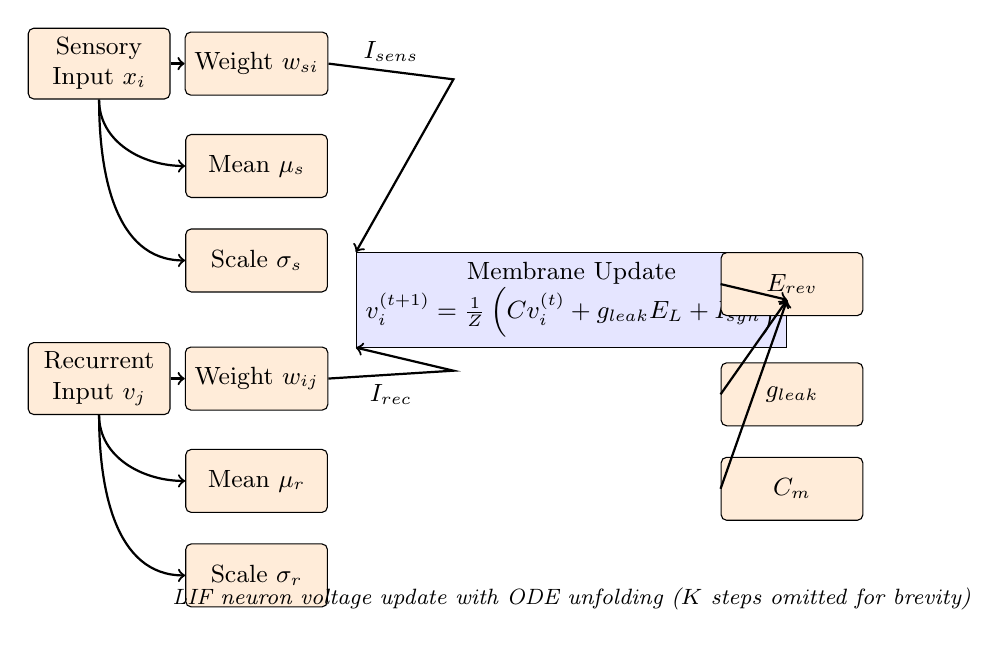
\begin{tikzpicture}[
    box/.style={draw, minimum height=1.2cm, minimum width=2.2cm, align=center, fill=blue!10},
    label/.style={font=\footnotesize\itshape},
    param/.style={draw, rounded corners=2pt, fill=orange!15, minimum height=0.8cm, minimum width=1.8cm, align=center},
    arrow/.style={->, thick},
    every node/.style={font=\small}
]

% Sensory Input
\node[param] (sens_input) at (-4, 2) {Sensory\\Input $x_i$};
\node[param] (sens_w) at (-2, 2) {Weight $w_{si}$};
\node[param] (sens_mu) at (-2, 0.7) {Mean $\mu_s$};
\node[param] (sens_sigma) at (-2, -0.5) {Scale $\sigma_s$};
\draw[arrow] (sens_input) -- (sens_w);
\draw[arrow] (sens_input.south) to[out=270,in=180] (sens_mu.west);
\draw[arrow] (sens_input.south) to[out=270,in=180] (sens_sigma.west);

% Recurrent Input
\node[param] (rec_input) at (-4, -2) {Recurrent\\Input $v_j$};
\node[param] (rec_w) at (-2, -2) {Weight $w_{ij}$};
\node[param] (rec_mu) at (-2, -3.3) {Mean $\mu_r$};
\node[param] (rec_sigma) at (-2, -4.5) {Scale $\sigma_r$};
\draw[arrow] (rec_input) -- (rec_w);
\draw[arrow] (rec_input.south) to[out=270,in=180] (rec_mu.west);
\draw[arrow] (rec_input.south) to[out=270,in=180] (rec_sigma.west);

% Central box: Membrane Voltage Update
\node[box] (voltage) at (2, -1) {Membrane Update\\ $v_i^{(t+1)} = \frac{1}{Z} \left(C v_i^{(t)} + g_\text{leak} E_L + I_{\text{syn}} \right)$};

% Arrows into voltage
\draw[arrow] (sens_w.east) -- (0.5, 1.8) node[midway, above] {$I_{\text{sens}}$} -- (voltage.north west);
\draw[arrow] (rec_w.east) -- (0.5, -1.9) node[midway, below] {$I_{\text{rec}}$} -- (voltage.south west);

% Leak + Capacitance
\node[param] (gleak) at (4.8, -2.2) {$g_\text{leak}$};
\node[param] (cm) at (4.8, -3.4) {$C_m$};
\node[param] (erev) at (4.8, -0.8) {$E_\text{rev}$};
\draw[arrow] (gleak.west) -- (voltage.east);
\draw[arrow] (cm.west) -- (voltage.east);
\draw[arrow] (erev.west) -- (voltage.east);

% Caption
\node[label] at (2, -4.8) {LIF neuron voltage update with ODE unfolding ($K$ steps omitted for brevity)};

\end{tikzpicture}
\caption{Internal structure of a single LIF neuron used in the Liquid Time-Constant Network. Inputs undergo non-linear transformations based on trainable $\mu$ and $\sigma$, with the resulting activations integrated using biophysical parameters such as leak conductance ($g_\text{leak}$), membrane capacitance ($C_m$), and reversal potentials ($E_\text{rev}$).}
\label{fig:lif_neuron_detailed}
\end{figure}


\hl{LTC ARCHITECTURE DIAGRAM HERE}

\section{Training Configuration (and dataset)}
The LNN was trained on a synthetic 2D spiral trajectory dataset, chosen for its smooth temporal structure and nonlinearity. Each data point consists of an $(x, y)$ coordinate, and the goal of the model is to predict the next point in the sequence given a fixed-length input window. The sequential nature of the task makes it well-suited for testing temporal memory and continuous dynamics.

A supervised learning approach was used; inputs and targets were created by shifting a sliding window of length $T = 3$ over the full spiral. Each input sequence of three time steps was paired with the corresponding next three steps as the target output.

\vspace{1em}
\noindent \textbf{Data Preprocessing:}
\begin{itemize}
    \item All inputs were standardised using the training set mean and standard deviation.
    \item Targets were normalised in the same way to preserve scale consistency.
    \item The spiral dataset was generated programmatically with adjustable number of points and turns.
\end{itemize}

\vspace{0.5em}
\noindent \textbf{Training Parameters:}
\begin{itemize}
    \item \textbf{Loss function:} Mean Squared Error (\texttt{nn.MSELoss()}) was used to penalise deviations from the ground truth trajectory.
    \item \textbf{Optimiser:} Adam was chosen due to its fast convergence and robustness to parameter scaling. The learning rate was set to 0.005.
    \item \textbf{Epochs:} The model was trained for 2000 epochs to ensure convergence, with periodic visual evaluation every 100 epochs.
    \item \textbf{Batching:} Input sequences were split into overlapping windows and grouped into batches of size 32. This batching strategy allowed efficient GPU utilisation while preserving temporal continuity.
    \item \textbf{Train/validation split:} A random 80/20 split was used, with shuffling applied to prevent memorisation of input order.
\end{itemize}

\vspace{1em}
\noindent Below is the training process implementation:
\begin{lstlisting}[language=Python, caption={Simplified training loop for the LNN}]
for epoch in range(num_epochs):
    lnn_model.train()
    total_loss = 0
    for x_batch, y_batch in zip(input_batches, target_batches):
        optimizer.zero_grad()
        outputs = lnn_model(x_batch)
        loss = criterion(outputs, y_batch)
        loss.backward()
        optimizer.step()
        total_loss += loss.item()
\end{lstlisting}

\vspace{0.5em}
\noindent The training loop includes evaluation checkpoints where predicted trajectories are plotted and compared to ground truth. These visualisations provided insights into convergence behaviour, beyond scalar loss values.

\vspace{1em}
\noindent \textbf{Implementation Details:}
\begin{itemize}
    \item A small sequence length ($T = 3$) was chosen to reduce training complexity while still allowing temporal dependencies to be captured.
    \item Training on a synthetically generated spiral ensured control over noise and resolution, which allowed clearer attribution of error sources to model limitations rather than data irregularities.
    \item The validation split was kept random to mimic real-world test generalisation, though later sections explore unseen spiral generation for more robust testing.
\end{itemize}

\section{Training Behaviour}
Throughout training, model performance was monitored both quantitatively (via validation loss) and qualitatively (through trajectory plots). Evaluation occurred at regular intervals (every 100 epochs), allowing for close inspection of how well the LNN was capturing the underlying dynamics of the spiral sequence.

\noindent The primary trends observed during training were:
\begin{itemize}
    \item Loss decreased steadily in early epochs, with diminishing returns as training progressed.
    \item In some cases, small fluctuations in validation loss were observed, likely due to the non-convexity of the parameter landscape and the biological variability induced by random wiring.
    \item Visual predictions of the trajectory showed clear improvement over time. Early predictions were coarse approximations, while later epochs yielded smoother and more accurate reconstructions.
\end{itemize}

\linebreakparagraph{Trajectory Loss Curves}

\noindent The following plot illustrates training and validation behaviour over time:

\begin{figure}[H]
    \centering
    \includegraphics[width=0.8\linewidth]{img/lnn_loss_curve.png}
    \caption{Training and validation loss over epochs.}
    \label{fig:lnn_loss}
\end{figure}

\begin{figure}[H]
    \centering
    \includegraphics[width=0.8\linewidth]{img/lnn_loss_curve_zoomed.png}
    \caption{Training and validation loss over epochs.}
    \label{fig:lnn_loss_zoomed}
\end{figure}

To evaluate the model's learning progress and generalisation, we record the full-sequence mean squared error (MSE) first on the entire spiral (which contains the training datapoint and the held-out validation datapoints), and then on a separate unseen evaluation spiral at each epoch. Rather than separately plotting training and validation loss — which are contiguous segments of the same spiral trajectory, they are treated as a single sequence. This is because since temporal continuity is essential in modelling dynamical systems. This decision avoids misleading interpretations that might arise from artificial segmentation of a naturally evolving system.

The resulting loss curves, shown in Figure~\ref{fig:lnn_loss} and Figure~\ref{fig:lnn_loss_zoomed}, allow a direct comparison of model performance on the trajectory it is optimised on versus a held-out trajectory generated under the same dynamics but seeded differently. Early in training, both curves decrease rapidly, suggesting that the model learns the underlying structure efficiently. As training proceeds, the two curves converge, with the evaluation spiral maintaining a slightly higher loss—indicating some generalisation gap but also demonstrating stable extrapolation beyond the training path. Notably, neither curve exhibits significant divergence or overfitting behaviour, which supports the robustness and consistency of the trained model.

\linebreakparagraph{Qualitative Evaluation}
Visually, the predicted path over time showed that the LNN was able to maintain smooth curvature and approximate the rotational dynamics of the spiral without overshooting or excessive lag. This was true even on validation data not seen during training. 

\begin{figure}[H]
    \centering
    \includegraphics[width=0.8\linewidth]{img/lnn_training_validation_spiral_epoch_1.png}
    \caption{LLN predicted vs true spiral trajectory at epoch 1, on denormalised training (and validation) spiral}
    \label{fig:lnn_training_validation_spiral_epoch_1}
\end{figure}

\begin{figure}[H]
    \centering
    \includegraphics[width=0.8\linewidth]{img/lnn_training_validation_spiral_epoch_400.png}
    \caption{LLN predicted vs true spiral trajectory at epoch 400, on denormalised training (and validation) spiral}
    \label{fig:lnn_training_validation_spiral_epoch_400}
\end{figure}

\begin{figure}[H]
    \centering
    \includegraphics[width=0.8\linewidth]{img/lnn_training_validation_spiral_epoch_2000.png}
    \caption{LLN predicted vs true spiral trajectory at epoch 2000, on denormalised training (and validation) spiral}
    \label{fig:lnn_training_validation_spiral_epoch_2000}
\end{figure}

\vspace{1em}
\noindent \textbf{Observed Patterns Across Training Runs:}
\begin{itemize}
    \item \textbf{ODE unfolding depth:} The number of internal steps in the membrane integration process contributed significantly to trajectory stability. Deeper unfolding improved smoothness, but with diminishing returns.
    \item \textbf{Effect of sparsity:} Fixed wiring helped constrain overfitting and may have contributed to better generalisation than a fully connected architecture.
    \item \textbf{Performance variation:} Some runs with different initialisations showed variability in loss curves and convergence speed, indicating sensitivity to initial wiring or parameter seeds.
\end{itemize}

Despite simpler architectures having shorter training times (e.g. LSTMs), LLN's had superior interprebility and stability in capturing the underlying continuous structure of the problem.

% TODO: Make sure this section is right & make it sound better

\subsection{Inference}

...

Although the models in this project were trained using fixed-size sliding windows (e.g., sequences of length 3 used to predict the next 3 points), inference is performed by passing the entire normalised input sequence to the model at once. Specifically, the inference function assumes that a model trained on short-range sequences can generalise to longer sequences when given a full trajectory (e.g., 199 input points to produce 199 output predictions). While this introduces a mismatch between training and inference regimes, the results obtained from this method---particularly on structured datasets such as smooth spiral trajectories---are stable, visually coherent, and achieve competitive prediction metrics.

This apparent generalisation is primarily due to the smooth, low-dimensional nature of the data. The spiral trajectories are continuous and predictable, and do not exhibit stochastic or chaotic behaviour. As a result, the models are able to extrapolate the learned local dynamics across the full trajectory during inference, even though they were not explicitly trained to do so.

Moreover, models like the Transformer and TCN use shared weights and position-aware mechanisms (such as causal convolutions or attention with position embeddings) that do not fundamentally restrict them to a fixed input length. Consequently, when exposed to longer sequences, these architectures can continue to apply the same learned local filters or attention patterns, leading to coherent global predictions. Importantly, since the full sequence of input data is provided during inference, there is no recursive feeding of the model's own outputs---avoiding the accumulation of compounding errors often seen in autoregressive inference.

Nonetheless, this approach is not universally applicable. On tasks with more complex temporal dependencies, discontinuities, or chaotic dynamics, such inference behaviour could lead to silent degradation in performance. For such settings, autoregressive inference---where predictions are generated step-by-step and recursively fed into the model---would be more appropriate, as it more closely matches the training distribution and better captures error propagation over time.

In this work, however, the use of full-sequence inference is empirically validated to be reliable on the spiral trajectory dataset, offering a clean and efficient method for evaluating models without significant performance degradation.
